% !TeX TS-program = xelatex

\documentclass{resume}
\ResumeName{田润泽的个人简历}

% 如果想插入照片,请使用以下两个库。
% \usepackage{graphicx}
% \usepackage{tikz}

\begin{document}

\ResumeContacts{
  (+86)186-2569-8616,%
  \ResumeUrl{mailto:trunzer@ruc.edu.cn}{trunzer@ruc.edu.cn},%
  \ResumeUrl{https://trunzer-world.cn}{trunzer-world.cn} \footnote{该网站正在维护。},%
  \ResumeUrl{https://github.com/Welldefine}{github.com/Welldefine}%
}

% 如果想插入照片,请取消此代码的注释。
% 但是默认不推荐插入照片,因为这不是简历的重点。
% 如果默认的照片插入格式不能满足你的需求,你可以尝试调整照片的大小,或者使用其他的插入照片的方法。
% 不然,也可以先渲染 PDF 简历,然后用其他工具在 PDF 上叠加照片。
% \begin{tikzpicture}[remember picture, overlay]
%   \node [anchor=north east, inner sep=1cm]  at (current page.north east) 
%      {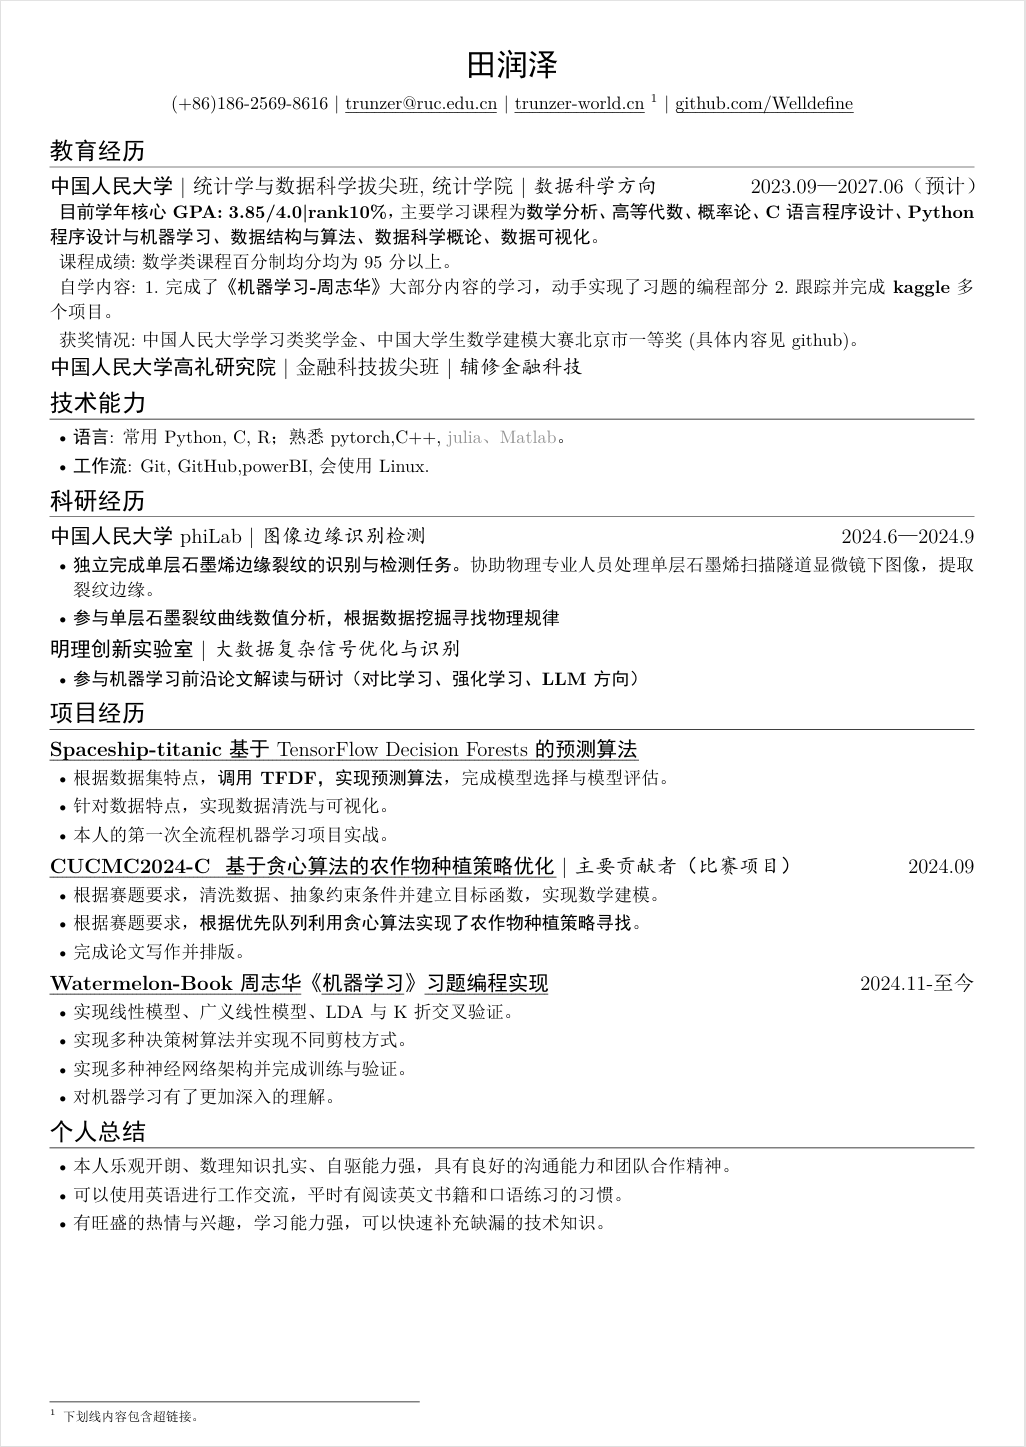
\includegraphics[width=2cm]{image.png}};
% \end{tikzpicture}

\ResumeTitle


\section{教育经历}
\ResumeItem
[中国人民大学|本科二年级在读]
{中国人民大学}
[\textnormal{统计学与数据科学拔尖班,统计学院|} 数据科学方向]
[2023.09—2027.06(预计)]

\textbf{目前学年核心GPA: 3.88/4.0},主要学习课程为\textbf{数学分析(100分)、高等代数(98分)、概率论(96分)、C语言程序设计、Python程序设计与机器学习、数据结构与算法}。

获奖情况:中国人民大学二等奖学金、2024中国大学生数学建模大赛北京市一等奖(具体内容见Github)、2025美国大学生数学建模大赛M奖(一等奖)。
\ResumeItem
{中国人民大学高礼研究院}[\textnormal{金融科技拔尖班|} 辅修金融科技]
\textbf{主修课程:} 微观经济学、货币金融学、宏观经济学、金融学实务、金融科技概论、商业技能

\section[技术能力]{技术能力\protect}
\begin{itemize}
  \item \textbf{语言}: 常用 Python, C ; 熟悉 pytorch, C, C++, \GrayText{julia,Matlab,blender}
  \item \textbf{工作流}: Git, GitHub, Linux(Ubuntu)
  \item $LaTeX$发烧友,熟练使用$LaTeX$排版,熟悉$Beamer$制作幻灯片
\end{itemize}

\section{科研经历}

\ResumeItem{中国人民大学phiLab}
[图像边缘识别检测——蔡鹏老师]
[2024.6—2024.9] 

\begin{itemize}
  \item \textbf{独立完成单层石墨烯边缘裂纹的识别与分类任务。}协助物理专业人员处理单层超导态石墨烯
  扫描隧道显微镜下图像,通过一维CNN实现超导体分类。
  \item \textbf{参与单层石墨裂纹曲线数值分析,根据数据挖掘寻找物理规律}
\end{itemize}

\ResumeItem{中国人民大学明理创新实验室}
[大数据复杂信号优化与识别——尹健鑫老师]
[2024.10—2025.3] 
\begin{itemize}
  \item \textbf{参与机器学习前沿论文解读与研讨(对比学习、强化学习、LLM方向)}
  \item \textbf{参与图像识别与生成式模型架构构建工作}
\end{itemize}

\ResumeItem{清华大学\&字节跳动:SIA-LAB}
[GenModel 生成式人工智能——分子生成任务]
[2025.6—至今]
\begin{itemize}
  \item \textbf{掌握Diffusion Model、ScoreModel、FLowModel、Bayesian FLow Network等生成式模型的基本原理。}
  \item \textbf{复现多种生成式模型,小规模分子生成模型的训练与测试。}
  \item \textbf{参与分子生成模型的代码优化与性能提升工作。}
\end{itemize}


\section{项目、比赛经历}

\ResumeItem[CUCMC2024-C 基于贪心算法的农作物种植策略优化]
{\ResumeUrl{https://github.com/Welldefine/CUMCM2024-C}{\textbf{CUCMC2024-C } 基于贪心算法的农作物种植策略优化}}
[主要贡献者(比赛项目)]
[2024.09]

\begin{itemize}
  \item 根据赛题要求,清洗数据、抽象约束条件并建立目标函数,实现数学建模。
  \item 根据赛题要求,\textbf{根据优先队列利用 贪心算法 实现了农作物种植策略寻找}。
  \item 完成论文写作并排版。
\end{itemize}

\ResumeItem[COMAP-ICM-E The Cascading Effects of
 Ecological Transition and Organic Agriculture]
{\ResumeUrl{}{\textbf{COMAP-ICM-E } 农田生态系统的动力学与有机农业的级联效应}}
[主要贡献者(比赛项目)]
[2025.01]
\begin{itemize}
  \item 根据赛题要求,清洗数据、抽象约束条件并建立目标函数,实现数学建模。
  \item 根据赛题要求,\textbf{利用微分方程与数值方法实现了农田生态系统的动力学模型}。
  \item 完成论文写作并排版。
\end{itemize}


\section{实习经历}
\ResumeItem[Intime AI虚实科技算法组]
{\ResumeUrl{https://www.intimeai.cn/}{\textbf{Intime AI虚实科技算法组}}}
[]
[2025.1-2025.6]
\begin{itemize}
  \item 3D生成模型的部署、测试与pipeline搭建
  \item 参与大规模3D资产数据集的构建、清洗与标注工作
  \item 实现多个模型api的部署与MCP服务的部署
  \item 参与使用深度学习参数化建模3D资产大模型算法的研讨与实现
\end{itemize}


\section{个人总结}

\begin{itemize}
  \item 本人乐观开朗、数理知识扎实、自驱能力强,具有良好的沟通能力和团队合作精神。
  \item 可以使用英语进行工作交流,平时有阅读英文书籍和口语练习的习惯。
  \item 有旺盛的热情与兴趣,学习能力强,可以快速补充缺漏的技术知识。
\end{itemize}


\end{document}
